\documentclass[11pt,twoside,a4paper]{article}
\usepackage{a4wide,amsmath,amssymb}
\usepackage[british]{babel}
\usepackage[utf8x]{inputenc}
\hyphenation{}

% Build pdf:
% $ pdflatex seminar_template.tex
% $ pdflatex seminar_template.tex
% Run pdflatex twice to get the references right...


%-------------------------- Formatting --------------------------%

% Picture and table title formats
\usepackage[bf,small]{caption}

\usepackage{enumitem}
\usepackage{listings}
\usepackage{longtable}
\usepackage{graphicx}

%\usepackage{mathpazo}  % -- use Palatino --
%\usepackage{mathptmx}  % -- or Times --

% Use this to discern DRAFTs from final versions
%\usepackage{draftcopy}
%\draftcopySetGrey{0.90}   %   90% = very light grey
%\draftcopySetScale{1}

%--------------- line and paragraph distances ----------------------%
\setlength{\parindent}{0em}
\setlength{\parskip}{\medskipamount}    % distance between paragraphs

% correctly format URLs and email addresses
\usepackage{url}
\usepackage{cite}
% example for email addresses: \url{foo@bar.com}

% Tools for note taking, ideas...
\newcommand{\notesubsection}[1][unsorted idea]{%
\subsection*{#1}%
\addcontentsline{toc}{subsection}{#1}%
}

% side note:
\newcommand{\bemerkung}[1]{\marginpar{\small\textsl{\textsf{#1}}}}

% this adds a little "under construction" icon on the side
%
% For this to work you need an "Baustelle.eps" icon. Get it from here:
%  http://www.net.in.tum.de/teaching/WS04/routing/Baustelle.eps.gz
\newcommand{\baustelle}[1][]{
 \marginpar{%
   \centerline{\includegraphics[scale=0.3]{Baustelle.eps}}
   {\small\textsl{\textsf{\raggedright #1}}}
}}

\begin{document}
\title{Weird Machines}
\author{Federico Scrinzi \\
  (\texttt{federico.scrinzi@campus.tu-berlin.de})\\[5mm]
  ``Computer Security Seminar" , \\
  Technische Universität Berlin
}
  
\date{WS\,2013/2014 (Version of \today)}

\maketitle

\abstract{
What are exploits in fact? It is possible to define them as programs that run on an unanticipated computational structure, performing unexpected computation. Buffer overflows, uncontrolled format strings or SQL injections are just few classical examples of vulnerabilities that allow to achieve this goal. It is possible to see exploits for these flaws as input data used as bytecode on some kind of virtual machine. We will call this class of peculiar VMs \emph{weird machines}.

Unexpected computation means not only the execution of unintended instructions on the CPU but can be achieved also using Turing complete machines hidden in the target. This paper will present two examples of weird machines: the first based on ABI metadata while the second on the MMU.
}


\section{Introduction}
Exploits are a proof-by-construction of unexpected computation. Through an exploit, what an attacker wants usually to achieve is to make the target machine do something that was not anticipated. Classically, this means deceiving the system into executing arbitrary code, but we will see that modern systems offer many different hidden ways of achieving computation.

In the last decade there was a major change in security analysis regarding this aspect: the threat model needed to be extended, from a simplistic approach based on "malicious code" to a more comprehensive one based on "malicious computation" \cite{hund}. 
The classic paper "Smashing the Stack for Fun and Profit" by Aleph One \cite{smashing} illustrates one of the first steps in the conversion of an input data flow into altered program control flow. Thus, not only code but also data may be a potential threat: data processing changes the state of the machine analyzing it, thus one could think of specially crafted inputs as a possible way to achieve computation \cite{noncontroldata}.

Modern systems hide a plethora of weird machines that might be exploited, the new goal for security analysts is to find them.   Turing-complete machines are hidden in many systems: CSS3 combined with HTML \cite{html}, C++ templates \cite{cpp_templates} or the Game of Life are proven to satisfy those properties. These are just a few examples of machines driven by what is not normally considered as executable code.

Therefore, security research's core subjects of study-trust and trustworthiness in computing systems are now faced with new questions, such as "What execution paths can programs be trusted to not take under any circumstances, no matter what the inputs?" or "Which properties of inputs can a particular security system verify, and which are beyond its limits?" \cite{bratus}.

This paper introduces two kind of weird machines: the first based on ELF metadata \cite{elf_machine} (Section 2), while the second on page faults and interrupt handling \cite{mmu_machine} (Section 3). Later, a brief comparison of these two constructions is presented (Section 4).

%Exploits based on weird machines are harder to detect than classical ones and hidden, unexpected computation can be a really dangerous threat. For that reason higher and higher consideration should be given to the study of this field, to reveal new potential hazard and build more secure systems.


\section{Weird machine \#1: ELF metadata construction}

This section presents the work of R. Shapiro, S. Bratus and S. W. Smith \cite{elf_machine} in building a weird machine that exploits ELF relocation metadata to achieve computation.

\subsection{Introduction to ELF}
The Executable and Linkable Format (ELF) is a file format for object code, executables and shared libraries. It is commonly used in many Unix-like systems such as Linux, *BSD and Solaris.
Each ELF file is composed by an ELF Header (metadata) followed by the actual data.

%There are three main types of object files:
%\begin{itemize}
%\item Relocatable files hold code and data suitable for linking with other object files to create an
%executable or a shared object file.
%\item Executable files hold a program suitable for execution.
%\item Shared object files holds code and data suitable for linking in two contexts. First, the link editor may process it with other relocatable and shared object files to create another object file. Second, the dynamic linker combines it with an executable file and other shared objects to create a process image.
%\end{itemize}
The loading and execution of a program can be summarized in the following steps \cite{eresi}:
\begin{enumerate}
\item The \texttt{exec()} system call is called with the path of the executable. The kernel takes control of the execution (\texttt{int \$0x80}) and reads a small subset of the executable's metadata in order to map the executable into memory and the executable's interpreter (typically the RTLD, \texttt{ld.so}) into the process' address space.
\item A context switch into userland is made and the interpreter is started (\texttt{RTLD\_START()} is called in the case of \texttt{ld.so})
\item The interpreter loads all the needed libraries such as \texttt{libc.so} and patches memory as specified by the executable's metadata
\item The execution jumps the executable's entry-point (usually \texttt{\_start})
\end{enumerate}

\subsubsection{Addresses relocation} 
%For our purposes the executable's metadata and the patching of the memory by the interpreter is particularly important, as the weird machine presented in this section is based on those primitives. We will go a bit more in detail in this step.

Unlike executables, when shared libraries are being built, the linker can not assume a known load address for their code. The reason for this is simple: each program can use any number of shared libraries, and there is simply no way to know in advance where any given shared library will be loaded in the process's virtual memory. This problem is solved by the RTLD.

The true entry point of the interpreter is \texttt{\_dl\_start}, this function is called by the kernel from the \texttt{start\_thread()} kernel function. At the end of the dynamic linking process, the starting function of the binary, the \texttt{\_start()} point, is called. \cite{eresi}

It is important to remark that every object in the dynamic linker is described by a \texttt{link\_map} structure. Those structures are only created at runtime and contain different kind of information, such as: the base address at which the ELF object was loaded, the virtual address of all the ELF object's dynamic table entries or pointers to other loaded link map structures. All the \texttt{link\_map} structures form a doubly linked list so from every structure we can find information on any other loaded ELF object by traversing the list.

Symbols are a way to assign mnemonic names to addresses. ELF provides two different symbol tables: \texttt{.symtab} and \texttt{.dynsym}. \texttt{.dynsym} is just a smaller version of the \texttt{.symtab} that only contains global symbols, it contains information required at runtime such as the names of the needed libraries. Symbol metadata is memorized using \texttt{Elf64\_Sym} structures. This kind of metadata is used in the following construction to build registers: symbols with 8 byte values are used, type must be set to \texttt{FUNC} so it is treated as a regular symbol. An example is the following: \begin{lstlisting}
{name=foo, value=0xb0000000, type=FUNC, shndx=1, size=8}
\end{lstlisting}

\texttt{.rela.dyn} and \texttt{.rela.plt} are two tables that contain relocation entries composed by structures of type \texttt{Elf64\_Rela}. Relocation entries are used to patch the table with the locations of imported library functions at runtime. The difference between the two tables is that \texttt{.rela.plt} entries are typically processed lazily during dynamic linking while \texttt{.rela.dyn} relocation entries are processed during load time, just before the RTLD passes control to the executable.

Three types of relocation entries are interesting for constructing the weird machine, they are shown in Table \ref{r_entries}.

\begin{table}
\centering
\begin{tabular}{ l | l }
  \hline
  \texttt{R\_X86\_64\_COPY} (COPY)
  &
\begin{lstlisting}
memcpy(r.offset,s.value,s.size)
\end{lstlisting} \\
  \texttt{R\_X86\_64\_64} (SYM) &
\begin{lstlisting}
*(base+r.offset)=s.value+
                 r.addend+base
\end{lstlisting} \\
  \texttt{R\_X86\_64\_RELATIVE} (RELATIVE) &
\begin{lstlisting}
*(base+r.offset)=r.addend+base
\end{lstlisting} \\
  \hline
\end{tabular}
  \captionsetup{width=13.5cm}
  \caption{ELF relocation entries that the weird machine uses. Their meaning is presented in C-like syntax where \texttt{r} is the relocation entry, \texttt{s} is the corresponding symbol and \texttt{base} is the base address of the ELF object.}
  \label{r_entries}
  \vspace{-0.4cm}
\end{table}


\subsection{Weird machine primitives}

The weird machine presented in this section implements a simplified assembly-like language. It offers the following instructions: move (\texttt{mov}), addition (\texttt{add}) and jump-if-not-zero (\texttt{jnz}). Accepted input formats for those instructions are:
\begin{itemize}
\item Immediate (e.g.: \texttt{\$0x42})
\item Direct, the given location contains the value address (e.g.: \texttt{*0xcafebabe})
\item Register, the given register contains the value (e.g.:\texttt{\%reg})
\item Register indirect, the given register contains the value address (e.g.: \texttt{[\%reg]})
\end{itemize}


\subsubsection{Move}
The \texttt{mov} instruction allows to copy a value from a source to a destination. It is trivial to build a \texttt{mov} instruction using relocation entries of type \texttt{RELATIVE}. The syntax of the instruction is:

\begin{lstlisting}
mov <dest>, <value>
\end{lstlisting}

Because of the structure of relocation entries \texttt{<dest>} has to be passed in direct mode while \texttt{<value>} supports either immediate or register indirect values. Figure \ref{mov_table} shows two examples of relocation entries that form a \texttt{mov} instruction.

\begin{figure}[ht]
\centering
\begin{tabular}{ l | l }
  \hline
\begin{lstlisting}
mov *0xbeef0000,
    $0x04
\end{lstlisting}
&
\begin{lstlisting}
{type=RELATIVE, offset=0xbeef0000,
 symbol=0, addend=0x04}
\end{lstlisting} \\
  \hline
\begin{lstlisting}
mov *0xbeef0000,
    [%foo]
\end{lstlisting}
&
\begin{lstlisting}
{type=COPY, offset=0xbeef0000,
 symbol=foo, addend=0}
\end{lstlisting} \\
  \hline
\end{tabular}
\caption{Examples of the conversion from a \texttt{mov} instruction to relocation metadata.}
\vspace{-0.4cm}
\label{mov_table}
\end{figure}

\subsubsection{Addition}
The \texttt{add} instruction allows to compute an addition and save the result to a destination. copy a value from a source to a destination. It is again trivial to build this instruction using \texttt{SYM} relocation entries. The syntax of the instruction is:

\begin{lstlisting}
add <dest>, <addend1>, <addend2>
\end{lstlisting}

Because of the structure of relocation entries  \texttt{<dest>} has to be specified as a direct value, \texttt{<addend1>} as a register value, and \texttt{<addend 2>} as an immediate value.

Figure \ref{add_table} shows an example of a relocation entry that forms an \texttt{add} instruction.

\begin{figure}[ht]
\centering
\begin{tabular}{ l | l }
  \hline
  \begin{lstlisting}
add *0xbeef0000,
    %foo, $0x02
  \end{lstlisting}
  &
  \begin{lstlisting}
{type=SYM, offset=0xbeef0000,
 symbol=foo, addend=2}
  \end{lstlisting} \\
  \hline
\end{tabular}
\caption{Example of the conversion from an \texttt{add} instruction to relocation metadata.}
\label{add_table}
\vspace{-0.4cm}
\end{figure}


\subsubsection{Jump-if-not-zero}
\texttt{jne} instructions allow to transfer the flow of execution to another point of the program. It is not easy to implement jumps using relocation entries, as, for their original purpose, there is no need for the interpreter to jump between them.

\paragraph{Building an unconditional jump.}
The processing of relocation addresses by the RTLD can be summarized with the following simplified code \cite{elf_machine}. For each \texttt{link\_map} structure (\texttt{lm}), the location (\texttt{lm->dyn[DT\_RELA]}) and size (\texttt{lm->dyn[DT\_RELASZ]}) of the object's relocation table are looked-up, then each relocation table entry is processed (with \texttt{relocate()}):
\begin{lstlisting}
while (lm != NULL) {
  r = lm->dyn[DT_RELA];
  end = r + lm->dyn[DT_RELASZ];
  for (; r < end; r++) {
    relocate(lm, r, &dyn[DT_SYM]);
  }
  lm = lm->prev;
}
\end{lstlisting}

The basic idea for building a jump is to modify \texttt{end} in order to exit the "for loop" prematurely without going on processing the following relocation entries, then enter in the "while loop" again but starting from a different \texttt{r}.
It is possible to achieve this by exploiting the RTLD behavior. These are the steps that have to be done:

\begin{enumerate}
\item Change \texttt{lm->prev} to point to the same relocation entry, so the while loop will process it again later (this, in the end, needs to be reset to the original value)
\item Set \texttt{lm->dyn[DT\_RELA]} to point to the relocation entry of the jump destination
\item Set \texttt{lm->dyn[DT\_RELASZ]} to the size of the relocation entries from the jump destination on
\item Change the value of \texttt{end} to exit the for loop
\end{enumerate}


The following summarizes the process needed to achieve each point.

\begin{itemize}
  \item[1.] A pointer to the \texttt{link\_map} is stored in the Global Offset Table (GOT), whose address is known at compile time. Thus, it is possible to compute the final address of \texttt{prev} and use a \texttt{mov} instruction to overwrite it. E.g.:
  \begin{lstlisting}
mov *<addr of prev>, $<addr of link_map>
  \end{lstlisting}
  \item[2-3.] For achieving this there is the requirement of knowing the virtual address of the dynamic table. It is possible to calculate it at compile time, again with \texttt{mov} instructions. E.g.:
  \begin{lstlisting}
mov *(<addr of DT_RELA>), <addr of next entry to process>
  \end{lstlisting}
  \item[4.] \texttt{end} is stored on the stack. If ASLR is turned on, its location is randomized. Luckily the loader stores the address of some stack-allocated data in a statically-allocated variable. We can lookup the base-address of the loader to calculate the location of this static variable. Assuming the
address of \texttt{end} is stored in a symbol called \texttt{sym-end}, the following instructions will set \texttt{end} to 0, forcing the loop to exit prematurely:
 \begin{lstlisting}
mov *<addr of next Rela's offset>, %sym-end
mov *<(value overwritten)>, $0
 \end{lstlisting}
\end{itemize}

\paragraph{Conditional branch.} To move from an unconditional branch to a conditional one there is the need of a bit more logic. For this feature we need to exploit the RTLD behavior with \texttt{IFUNC} type symbols: these structures are processed in two different ways, depending on the value of the \texttt{shndx} field. (1) If it is not 0, then the RTLD treats the symbol as an indirect function, calling the function it points to and using the returned value. (2) If the \texttt{shndx} field is zero, then that symbol's value is used directly.

For achieving our goal we need a special symbol (that we call \texttt{sym-zero}) that is of type \texttt{IFUNC} and points to a function that returns zero. Then we need the following instructions:
\begin{lstlisting}
mov *<addr of sym-zero shndx>, $<test val>
add *<addr of end>, %sym-zero, $0
\end{lstlisting}

In this way if the value being tested is zero, then also \texttt{\%sym-zero} will be treated as zero (because of the \texttt{IFUNC} processing), so \texttt{end} will be zero and the for loop will exit. Otherwise \texttt{end} will be greater than zero, so the following instruction, that resets \texttt{end} to its original value, will be executed and the computation will go on without branching.


\subsection{A Turing complete machine inside ELF}

Using the given primitives it is possible to achieve computation using only ELF relocation metadata. No code is injected in the binary, only more ELF headers are added, but still it is possible to execute instructions or modify memory before the actual code is executed. This approach is also robust against ASLR.

The original authors of the paper built a Brainfuck to ELF-metadata compiler to demonstrate how to practically awake the hidden weird machine in the RTLD.

This document will not explain implementation challenges and constraints, but, if the reader is interested, he can go into more detail by reading the original paper \cite{elf_machine}. However, here there are particular points that are important to keep in mind when implementing this weird machine:
\begin{itemize}
\item For implementing conditional branching there is the need to know the base address of the RTLD. This is not trivial.
\item Existing metadata should not be corrupted, we want the final executable to still run as normal.
\item The interpreter runs some sanity checks on the metadata, they should not corrupt the weird machine instructions.
\end{itemize}


\subsection{Where to go from here?}
This weird machine is heavily dependent upon ELF, probably other executables format can be exploited in the same way. For this reason also PE (Windows) and Mach-O (OSX) are a subject of future research.

The relocation-metadata machine also shows that executable headers must be taken into account when studying the security of a system and are worth to be analyzed in detail by antivirus systems.

To better explain how an attacker could exploit this weird machine the original authors built a root shell backdoor hidden in the relocation metadata of a \texttt{ping} executable \cite{ping_elf}. It is important to remark that: 
\begin{itemize}
\item Ping runs with the SUID bit but drops privileges 
\item The optional \texttt{--type} command-line argument is passed to the \texttt{strcasecmp} function.
\end{itemize}

To get ping to execute arbitrary programs as root, we have to insert relocation metadata to override the call to \texttt{setuid()} to not do anything useful (so privileges are not dropped) and the call to \texttt{strcasecmp} to launch a \texttt{execl} instead. It turns out that it can be implemented using nine relocation entries and one symbol table entry, without making any changes to the executable segments of ping.

%It is interesting to notice that is possible to achieve this even without all the power of Turing-completeness, hence an attacker might need very little power to exploit weird machines.

\section{Weird machine \#2: Page fault driven computation}
The goal of the weird machine presented in this section is to exploit the MMU to do computation \cite{mmu_machine}.
%This suggests that we could consider the internal logic of page fault and memory translation as the finite automaton of a Turing machine and the memory as holding its "tape", by potentially creating a kind of a closed loop of memory accesses.

Interrupt handling and address translations are controlled using registers and tables, moreover, when a page fault occurs the information about the trap is saved on the stack. By setting the address of the trap handler to cause another fault we will end up with the processor continuously dispatching page-faults. If the tables controlling this behavior are crafted in the right way, the side effects of the interrupt handling form a Turing-complete one-instruction computer.

\subsection{Introduction to MMU and trap handling}

In order to understand MMU and trap handling a set of definitions is presented \cite{intel}.

%\paragraph{MMU: } Memory management unit, it is an hardware component responsible for handling accesses to memory requested by the CPU. Among other features it is in charge of translating virtual addresses to physical addresses.

\paragraph{TSS: } Task state segment, it is a special structure which holds information about a task. Specifically, it contains: registers' state, I/O port permissions, inner-level stack pointers, previous TSS link. The CPU has hardware features that allow saving the entire state to a TSS and restoring it from there. Therefore, it is possible to switch between contexts with a single instruction or interrupt without any further logic.

\paragraph{TR: } Task register, it is a register that contains the selector for the "current" task state segment. Whenever the CPU switches to a different task it will save its state to the TSS stored in TR.

\paragraph{IDT: } Interrupt descriptor table, it is a data structure used by the CPU to determine the correct response to interrupts and traps. Every interrupt handler references a TSS descriptor in the GDT.

\paragraph{GDT: } Global Descriptor Table, it contains segment descriptors. The CPU addresses memory through an index into the GDT, called \texttt{segment selector} and an offset into the resulting interval.

\paragraph{Page fault: } A page fault occurs when a program requests an address on a page that is not in the current set of memory resident pages. Usually the OS tries to handle the page fault calling the specific handler in the IDT. It should make the required page accessible at a location in physical memory or terminate the program in the case of an illegal access.


\subsubsection{X86 interrupt handling}

The following summarizes how an interrupt is handled by the OS on x86 \cite{intel}.

\begin{enumerate}
\item An interrupt is raised
\item The current task is saved in the TSS pointed by the TR
\item The IDT is looked up for the right handler for the interrupt (every type of interrupt has a different handler). The handler is a pointer to a TSS descriptor in the GDT
\item The new TSS is loaded to handle the fault
\item The stack pointer is decremented by 4 and the information about the interrupt is written on the stack by the CPU
\end{enumerate}

\subsection{Weird machine primitives}

The only instruction we need to build is called \texttt{movdbz}, that stands for "move-branch-if-zero-or-decrement".

\texttt{movdbz <dest> <source> <branch>}

This construction is proven to be Turing complete \cite{mmu_machine}, its behavior is summarized as follows:
\begin{enumerate}
\item \texttt{source} is loaded and decremented
\item if the decrementation did not cause an underflow the result is stored in \texttt{dest} and the computation flow goes on to the next instruction
\item otherwise, if the decrementation caused an undeflow, 0 is stored in \texttt{dest} and the program flow jumps to \texttt{branch}
\end{enumerate}

For the construction of the weird machine the following components are needed:
\begin{itemize}
\item one specially crafted GDT
\item one TSS for each instruction
\item one page table per instruction (the memory is remapped, depending on the instruction)
\end{itemize}

The original authors built a compiler that converts \texttt{movdbz} instructions to these components \cite{trapcc}.

This is the pseudocode of the algorithm we want to execute, with a brief explanation of how to achieve this using only the MMU:
\begin{lstlisting}
Label:        # jump here through a PF or a DF
  X = Y       # save the old TSS state and load a new one
  if X < 4:   # try to decrement SP
    goto B    # if it caused an underflow we get a DF (jump)
  else:
    X -= 4    # SP decremented successfully
    goto A    # EIP will cause another PF
\end{lstlisting}


\subsection{A Turing complete machine based on Page Faults}

The following schema summarizes the lifecycle of the weird machine.

\begin{enumerate}
\item A page fault (or a double fault) is raised
\item The page fault (or the double fault) handler is looked-up in the IDT. A task switch is made: the current TSS is saved in the descriptor pointed by the TR, a new TSS is loaded.
\item The TSS contains, among other data, the registers state. The most interesting registers for the weird machine are ESP and CR3 (pointer to the page table). The first one plays the role of \texttt{X} in the pseudocode while the latter is used to remap the same virtual addresses into different physical addresses, by using a different page table.
\item The CPU tries to decrement ESP, in order to write information about the fault on the stack. If ESP is greater-or-equal than 4 the operation succeeds, however, this will raise another page fault as EIP points to an invalid address. Vice-versa, if ESP is lower than 4 we obtain an underflow that leads to a double fault.
\item The "execution" goes back to point 1. It is hence important to remark that now we have a different page table than before (because of a different value in CR3). So, because of how the tables were crafted, the IDT entries for the PF or the DF will now point to a different TSS. Moreover, also the address in the TR will point to another TSS, so the modified state will be saved in the next instruction.
\end{enumerate}

\begin{figure}[ht]
\centering
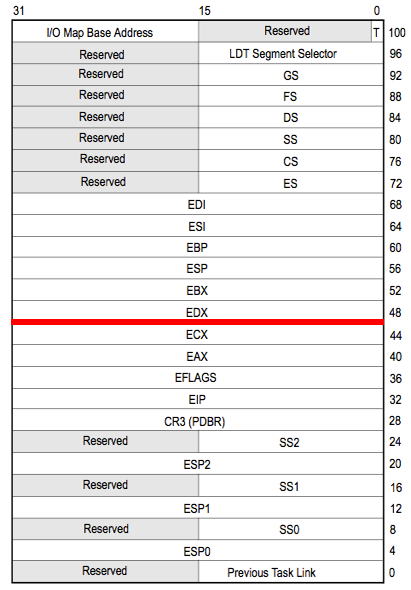
\includegraphics[scale=0.30]{tss.png}
\captionsetup{width=13.5cm}
\caption{The TSS is placed on a page boundary: by playing with page tables, when saving the state, the upper part will point to the physical address of the next TSS while the lower part will point to a GDT entry (to clear the \emph{busy-bit}) \cite{intel}
}
\label{TSS_fig}
\end{figure}

This description, however, is a little simplified. There are many constraints and implementation issues that are not covered by this paper, refer to the original one for more information \cite{mmu_machine}. These are few examples:
\begin{itemize}
\item By placing the TSS on a page boundary only the upper part of the table is saved in the "next instruction" (i.e. the next TSS) to keep the ESP state. The lower part, that contains the CR3 register, is not changed. See Figure \ref{TSS_fig}.
\item When an instruction is executed the CPU sets the \emph{busy bit} in the GDT, therefore it is not possible to jump back to that instruction without resetting the bit.
\item It is not possible to switch to the same task pointed by the TR
\item triple faults cause the machine to reboot, so they must be avoided
\end{itemize}


\subsection{Conclusions}
This weird machine shows a new and completely unexpected way to achieve computation.
It is important to remark that, for executing "instructions" on this machine, we do not actually compute any real instruction on the CPU. Everything is handled by the MMU. 

An interesting fact is that it is possible to switch between the weird machine and real instructions very easily: the only thing we need to do is to set EIP properly, in order not to cause a page fault. A proof of this is given by the original authors, as they built a "Game of Life" that runs computation on the MMU but switches to real instructions to display the gliders in the terminal.


\section{Comparison of weird machines \#1 and \#2}

The two weird machines presented in this document are very different but both achieve the same goal: unexpected computation in a totally unanticipated way. 
This opens to new techniques of hiding malware and new approaches to malware analysis.

A brief comparison of advantages and disadvantages of each machine is presented in Figure \ref{advantages} and \ref{disadvantages}.

\begin{figure}[ht!]
\begin{longtable}{ p{0.40\textwidth} | p{0.40\textwidth} }
\bfseries{ELF metadata weird machine} & \bfseries{MMU weird machine} \\ \hline
\begin{itemize}[noitemsep,topsep={0pt},partopsep={0pt}]
\item Metadata is not usually considered harmful, most defenses focus on actual code
\item Metadata is not always considered when signing executables
\item Not influenced by ASLR
\item The code is untouched
\item The weird machine metadata is still well formed, it does not fail any sanity check
\item ELF metadata can locate stack and all mapped libraries, redirect library calls or even perform function calls
\vspace{-0.6cm}
\end{itemize}
&
\begin{itemize}[noitemsep,topsep={0pt},partopsep={0pt}]
\item No native instruction needed for computation
\item Can be extremely difficult to detect and to analyze what it is actually computing
\item Possible to switch between weird machine and real instructions almost transparently
\item Exploits only hardware features, no further logic needed
\vspace{-0.6cm}
\end{itemize}
\end{longtable}
\caption{Advantages of the given constructions}
\vspace{-0.8cm}
\label{advantages}
\end{figure}


\begin{figure}[ht!]
\vspace{-0.1cm}
\begin{longtable}{ p{0.40\textwidth} | p{0.40\textwidth} }
\bfseries{ELF metadata weird machine} & \bfseries{MMU weird machine} \\ \hline
\begin{itemize}[noitemsep,topsep={0pt},partopsep={0pt}]
\item Runs native instructions, computation is not so hidden
\item Implementation specific for a version of \emph{glibc}, could easily break with other versions
\item Not possible to switch between weird machine and "normal" execution
\vspace{-0.6cm}
\end{itemize}
&
\begin{itemize}[noitemsep,topsep={0pt},partopsep={0pt}]
\item Needs kernel access to setup the components (GDT, IDT, TSSs, etc...)
\item Can only use the \texttt{movdbz} instruction: very minimalistic and not practical
\item Because of implementation issues it can only work with ESP of TSSs aligned across pages. This leads to a very limited coverage of physical memory
\item Need to insert dummy instructions to not have triple faults
\vspace{-0.6cm}
\end{itemize}
\end{longtable}
\caption{Limitations of the given constructions}
\vspace{-0.6cm}
\label{disadvantages}
\end{figure}


\section{Conclusions}

The study of trustworthiness of computing systems is typically predicated on assurance regarding the types of computation these systems can and cannot be driven: this machines show that there are many grey areas in this field that need more work and analysis.
These results demonstrate that special crafting of ELF metadata can lead to the execution of instruction on the CPU and modifications of the memory, moreover the unorthodox use of MMU features in modern processors can result in powerful computation, driven entirely by in-memory descriptor tables without dispatching any native instructions.

These observations lead to new questions in the field of trusted systems and, hopefully, encourage new efforts in research, in order to enumerate and characterize other unexpected computational environments.

\bibliographystyle{plain}
\bibliography{bibliography}

\end{document}

